%保存为UTF-8编码格式
%用xelatex编译
 
\documentclass[UTF8,a4paper,12pt]{ctexart}
\usepackage[left=2.50cm, right=2.50cm, top=2.50cm, bottom=2.50cm]{geometry} %页边距
\CTEXsetup[format={\Large\bfseries}]{section} %设置章标题字号为Large,居左
%\CTEXsetup[number={\chinese{section}}]{section}
%\CTEXsetup[name={(,)}]{subsection}
%\CTEXsetup[number={\chinese{subsection}}]{subsection}
%\CTEXsetup[name={(,)}]{subsubsection}
%\CTEXsetup[number=\arabic{subsubsection}]{subsubsection}  %以上四行为各级标题样式设置,可根据需要做修改
 
\linespread{1.25} %设置全文行间距
 
 
%\usepackage[english]{babel}
%\usepackage{float}     %放弃美学排版图表
\usepackage{fontspec}   %修改字体
\usepackage{amsmath, amsfonts, amssymb} % 数学公式相关宏包
\usepackage{color}      % color content
\usepackage{graphicx}   % 导入图片
\usepackage{subfigure}  % 并排子图
\usepackage{url}        % 超链接
\usepackage{bm}         % 加粗部分公式,比如\bm{aaa}aaa
\usepackage{multirow}
\usepackage{booktabs}
\usepackage{epstopdf}
\usepackage{epsfig}
\usepackage{longtable}  %长表格
\usepackage{supertabular}%跨页表格
\usepackage{algorithm}
\usepackage{algorithmic}
\usepackage{changepage}
\usepackage{listings}
\usepackage{xcolor}
 
\lstset{
    numbers=left, 
    numberstyle= \small, 
    keywordstyle= \color{ blue!70},%设置关键字颜色
    commentstyle= \color{red!50!green!50!blue!50}, %设置注释颜色
    frame=shadowbox, % 阴影效果
    rulesepcolor= \color{ red!20!green!20!blue!20} ,
    escapeinside=``, % 英文分号中可写入中文
    xleftmargin=2em, %距离左边界2em
    aboveskip=1em,
    framexleftmargin=2em,
    basicstyle=\ttfamily,
    columns=fullflexible,%可以自动换行
    linewidth=1\linewidth, %设置代码块与行同宽
    breaklines=true,%在单词边界处换行。
    showstringspaces=false,%去掉空格时产生的下划的空格标志, 设置为true则出现
    breakatwhitespace=ture,%可以在空格处换行
    escapechar=`%设置转义字符为反引号
}
 
%%%%%%%%%%%%%%%%%%%%%%%
% -- text font --
% compile using Xelatex
%%%%%%%%%%%%%%%%%%%%%%%
% -- 中文字体 --
%\setCJKmainfont{Microsoft YaHei}  % 微软雅黑
%\setCJKmainfont{YouYuan}  % 幼圆
%\setCJKmainfont{NSimSun}  % 新宋体
%\setCJKmainfont{KaiTi}    % 楷体
\setCJKmainfont{SimSun}   % 宋体
%\setCJKmainfont{SimHei}   % 黑体
 
% -- 英文字体 --
\setmainfont{Times New Roman}
%\setmainfont{DejaVu Sans}
%\setmainfont{Latin Modern Mono}
%\setmainfont{Consolas}
%
%
\renewcommand{\algorithmicrequire}{ \textbf{Input:}}     % use Input in the format of Algorithm
\renewcommand{\algorithmicensure}{ \textbf{Initialize:}} % use Initialize in the format of Algorithm
\renewcommand{\algorithmicreturn}{ \textbf{Output:}}     % use Output in the format of Algorithm
\renewcommand{\abstractname}{\textbf{\large {摘\quad 要}}} %更改摘要二字的样式
\newcommand{\xiaosi}{\fontsize{12pt}{\baselineskip}}     %\xiaosi代替设置12pt字号命令,不加\selectfont,行间距设置无效
\newcommand{\wuhao}{\fontsize{10.5pt}{10.5pt}\selectfont}
 
\usepackage{fancyhdr} %设置全文页眉、页脚的格式
\pagestyle{fancy}
\lhead{}           %页眉左边设为空
\chead{}           %页眉中间
\rhead{}           %页眉右边
%\rhead{\includegraphics[width=1.2cm]{1.eps}}  %页眉右侧放置logo
\lfoot{}          %页脚左边
\cfoot{\thepage}  %页脚中间
\rfoot{}          %页脚右边
 
 
%%%%%%%%%%%%%%%%%%%%%%%
%  设置水印
%%%%%%%%%%%%%%%%%%%%%%%
%\usepackage{draftwatermark}         % 所有页加水印
%\usepackage[firstpage]{draftwatermark} % 只有第一页加水印
% \SetWatermarkText{Water-Mark}           % 设置水印内容
% \SetWatermarkText{\includegraphics{fig/ZJDX-WaterMark.eps}}         % 设置水印logo
% \SetWatermarkLightness{0.9}             % 设置水印透明度 0-1
% \SetWatermarkScale{1}                   % 设置水印大小 0-1
 
\usepackage{hyperref} %bookmarks
\hypersetup{colorlinks, bookmarks, unicode} %unicode
 
 
\title{\textbf{\LARGE{Lab3 Report}}}
\author{涂宇清}
\date{5220309101520}
 
 
 
\begin{document}
 
\maketitle
%\tableofcontents

\setcounter{page}{1}        %从下面开始编页,页脚格式为导言部分设置的格式
 
 
\section{The control logic}
In order to realize the functions of the LC-3 simulator, we need to implement the simulation routine on the basis of the shell provided. Therefore, we need to implement six stages of an instruction cycle: fetch instructions, decode, evaluate address, fetch operands, execute and store results.

\section{Important function}
\subsection{Fetch instructions}
In order to complete the function of fetching instructions, we use\\
\verb|int instr = MEMORY[CURRENT_LATCHES.PC];| to get the instruction in the memory. Then we need to update the value of the PC, so we use \verb|NEXT_LATCHES.PC = CURRENT_LATCHES.PC + 1;| to update the value of the PC.

\subsection{Decode}
To decode the instruction, we need to get the opcode and the other parts of the instruction. \verb|int opcode = (instr & 0xF000) >> 12;| can get the opcode of the instruction. Then we use \verb|switch (opcode)| to judge the type of the instruction.

\subsection{Evaluate address}
Before evaluating the address, we need to determine the addressing mode (PC-relative, base register, or indirect). Then we can get the address of the operand. 

\subsection{Fetch operands}
To fetch the operands, we need to get the value of the register. We can use\\
\verb|CURRENT_LATCHES.REGS[sr];| to get the value of the register.

\subsection{Execute}
Once we have the address and operand, we only need to follow the ISA to execute.

\subsection{Store results}
After executing the instruction, we need to store the results. We can use\\
\verb|NEXT_LATCHES.REGS[dr] = result;| to store the results.

\subsection{SEXT}
The SEXT function is used to sign-extend the n-bit offset to 16 bits. We can use the following macro definition to implement this feature:

\begin{lstlisting}
#define SEXT(x, n) (x << 32-n >> 32-n)
\end{lstlisting}

\subsection{Set condition codes}
When we execute some instructions (such as ADD, AND, NOT, LD, LDI, LDR), we need to set the condition codes. We can use the following function to set the condition codes:

\begin{lstlisting}
void SetCC(int dr){
    int sign = (NEXT_LATCHES.REGS[dr] & 0x8000) >> 15;
    if (sign){
        NEXT_LATCHES.N = 1;
        NEXT_LATCHES.Z = 0;
        NEXT_LATCHES.P = 0;
    }
    else if (NEXT_LATCHES.REGS[dr] == 0){
        NEXT_LATCHES.N = 0;
        NEXT_LATCHES.Z = 1;
        NEXT_LATCHES.P = 0;
    }
    else {
        NEXT_LATCHES.N = 0;
        NEXT_LATCHES.Z = 0;
        NEXT_LATCHES.P = 1;
  }
}
\end{lstlisting}

\section{The verification of LC-3 simulator}

To verify this LC-3 simulator, we can compare its output with the simulator's output used in Lab1 and Lab2.

\subsection{Calculate the Fibonacci sequence}

In the first test, we calculate $f(n)$ in Fibonacci sequence. $n$ is in memory location x3000. The result is stored in memory location x3014, $f(n)$ is in memory location x3015. The result is as follows:

\begin{figure}[H]   %*表示可跨栏,如果不需要可去掉
\centering
\subfigure[The result of my LC-3 simulator]{
 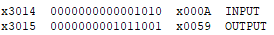
\includegraphics[width=0.5\textwidth]{Fibonacci1.png}}
 \hspace{0.2cm}      %两张图片之间的距离
%\hfill               %撑满整行
\centering
\subfigure[The result of the simulator used in Lab1 and Lab2]{
 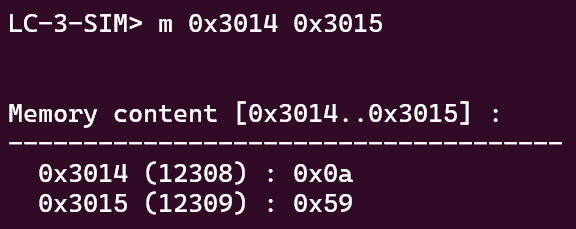
\includegraphics[width=0.4\textwidth]{Fibonacci2.png}}
\caption{The comparison of results}
\end{figure}

The outputs of both simulators is the same, and both are the tenth item in the Fibonacci sequence (decimal 89).

\subsection{Shift the binary number right}

In the second test, we shift the binary number right $n$ bits. The binary number is stored in memory location x301b,  $n$ is stored in memory location x301f, and The result is stored in memory location x3100. The result is as follows:

\begin{figure}[H]   %*表示可跨栏,如果不需要可去掉
\centering
\subfigure[The inputs of my LC-3 simulator]{
    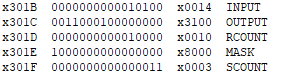
\includegraphics[width=0.5\textwidth]{shift1.png}}
    \hspace{0.2cm}      %两张图片之间的距离
%\hfill               %撑满整行
\centering
\subfigure[The inputs of the simulator used in Lab1 and Lab2]{
    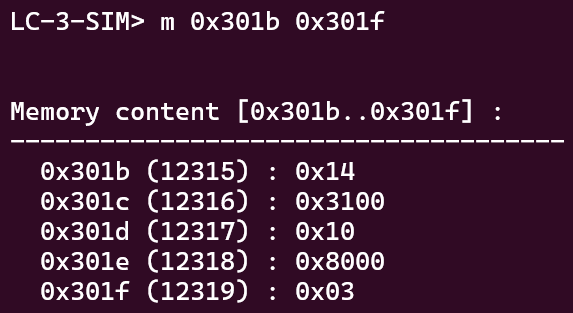
\includegraphics[width=0.4\textwidth]{shift3.png}}
\caption{The comparison of inputs}
\end{figure}

\begin{figure}[H]   %*表示可跨栏,如果不需要可去掉
\centering
\subfigure[The result of my LC-3 simulator]{
    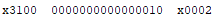
\includegraphics[width=0.5\textwidth]{shift2.png}}
    \hspace{0.2cm}      %两张图片之间的距离
%\hfill               %撑满整行
\centering
\subfigure[The result of the simulator used in Lab1 and Lab2]{
    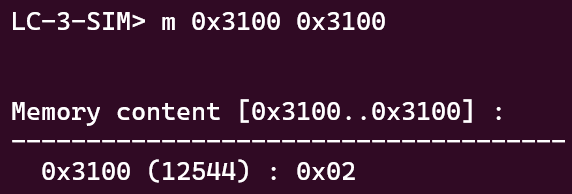
\includegraphics[width=0.4\textwidth]{shift4.png}}
\caption{The comparison of results}
\end{figure}

The outputs of both simulators is the same, and both are the result of shifting the input binary number right 3 bits.

\subsection{Conclusion}

Through two controlled experiments, we can see that the output of my LC-3 simulator is the same as the simulator used in Lab1 and Lab2. Therefore, we can conclude that the LC-3 simulator is correct.
 
\end{document}